%\documentstyle[epsf,twocolumn]{jarticle}       %LaTeX2e仕様
\documentclass[twocolumn]{jarticle}     %pLaTeX2e仕様(platex.exeの場合)
%\documentclass[twocolumn]{ujarticle}     %pLaTeX2e仕様(uplatex.exeの場合)
%%%%%%%%%%%%%%%%%%%%%%%%%%%%%%%%%%%%%%%%%%%%%%%%%%%%%%%%%%%%%%
%%
%%  基本バージョン
%%
%%%%%%%%%%%%%%%%%%%%%%%%%%%%%%%%%%%%%%%%%%%%%%%%%%%%%%%%%%%%%%%%
\setlength{\topmargin}{-45pt}
%\setlength{\oddsidemargin}{0cm} 
\setlength{\oddsidemargin}{-7.5mm}
%\setlength{\evensidemargin}{0cm} 
\setlength{\textheight}{24.1cm}
%setlength{\textheight}{25cm} 
\setlength{\textwidth}{17.4cm}
%\setlength{\textwidth}{172mm} 
\setlength{\columnsep}{11mm}

\kanjiskip=.07zw plus.5pt minus.5pt


% 【節が変わるごとに (1.1)(1.2) … (2.1)(2.2) と数式番号をつけるとき】
%\makeatletter
%\renewcommand{\theequation}{%
%\thesection.\arabic{equation}} %\@addtoreset{equation}{section}
%\makeatother

%\renewcommand{\arraystretch}{0.95} 行間の設定

%%%%%%%%%%%%%%%%%%%%%%%%%%%%%%%%%%%%%%%%%%%%%%%%%%%%%%%%
\usepackage[dvipdfmx]{graphicx}   %pLaTeX2e仕様(\documentstyle ->\documentclass)\documentclass[dvipdfmx]{graphicx}
\usepackage[subrefformat=parens]{subcaption}
%%%%%%%%%%%%%%%%%%%%%%%%%%%%%%%%%%%%%%%%%%%%%%%%%%%%%%%%

\begin{document}

\twocolumn[
\noindent

\hspace{1em}
\today
\hfill
\ \ 細川 岳大

\vspace{2mm}

\hrule

\begin{center}
{\Large \bf 進捗報告}
\end{center}
\hrule
\vspace{3mm}
]

% ‚ここから 文章 Start!
\section{今週やったこと}
 GAを用いたDataAugmentaion

\section{実験1}
前回に引き続きGAを用いたDataAugmentationの実験を行った.\\
変更点は各transformの適応確率を0\%から100\%まで10\%ずつ計11段階を導入した.\\
また,強度の遺伝子について前回までは0から5をとり,その強度に[-1,1]のランダムな値をかけて適用強度としていたが,
transformのランダム性を取り除きまた,一部において負の変換
(例えばrotateであれば90°の回転にいたいし時計回りと反時計回りがある)を考慮し-5から5をとるものとした.


\subsection{実験データ}
実験データはcifar10を用いて,
事前学習ではepoch数300,train\_dataを各ラベル5000枚の計50000枚使用し,GAで学習する際はepoch数100,train\_dataは各ラベル200枚のオリジナルとそれらすべてをDataAugmentaionしたものとを合わせ計4000枚とし,test\_dataは共に10000枚とした.また事前学習でのaccuracyは0.8475である.
\subsection{遺伝的アルゴリズム}


\subsubsection{探索空間}
\ 探索する水増し操作として画素値操作(Sharpness,Posterize,Brightness,Autoconstrast,Equalize,Solarize,Invert,Contrast,ColorBalance),
変形操作(Mirror,Flip,Translate X/Y,Shear X/Y,Rotate)の16種類の操作であり,今回はそれらすべてを個別にどの程度強くかけるかおよびどの順序でかけるかということを探索する.各操作についての強度の最大最小を設定し,それを-100\%から100\%まで25\%ずつ分11段階の度合いとする.ただし,Autocontrast,Equalize,Invert,Mirror については適用するか否かであるためパラメータが0以上で適用するとした.強度は0から5の整数値を持つ15個の遺伝子を実数値コーディングによって表現する.
また,適用順序に関しては同様に15個の遺伝子を持つ順列コーディングによって表現する.
確率は10\%ごと11段階の実数地コーディングによって表現する.
つまり,探索空間は$2^5*11^{11}*15!*11^{16}$となる.

\subsubsection{選択}
\ 選択について,エリート選出によって最も適応度の高い2つの個体を選択する.なお,この二つは後述する交叉,突然変異は受けずに次の世代に追加する.
残りの選出にはトーナメント選出を用した.トーナメント選出は集団の中から任意の数(トーナメントサイズ)の個体のうち最も適応度の高い個体を選出し次の世代に追加する.今回トーナメントサイズは2とした.
 
\subsubsection{交叉}
\ 強度,確率を表す染色体については2点交叉,順序を表す染色体については部分写像交叉を用いた.2点交叉は一対の親染色体をそれぞれ同じ場所で三分割し中央の染色体を入れ替えて交叉を行う.部分写像交叉は親遺伝子を二分割し入れ替える際重複をなくす交叉法で,重複のあった遺伝子について,それに該当した重複する遺伝子座を見つけ,それに対となっているもう一方の親の遺伝子を参照する.
 
\subsubsection{突然変異}
\ 強度,確率を表す染色体について,対象となる遺伝子の値を各50\%の確率に1増減させ,
 順序を表す染色体について,染色体の一部を逆順にする操作か,染色体を二つに分け前後を入れ替える操作のいずれかを行うものとした.
 
\subsection{パラメータ}
表\ref{tb:param}に学習パラメータを示す.
\begin{table}[h]
	\centering
	\caption{学習パラメータ\label{tb:param}}
	\scalebox{1.0}{
		\begin{tabular}{|c||c|} \hline
			optimizer&Adam\\ \hline
			learning rate&0.001\\ \hline
			loss function&categorical\_crossentropy\\ \hline
			batch size&128\\ \hline
		\end{tabular}
	}
\end{table}
 表\ref{tb:param1}にGAの設定を示す.
\begin{table}[h]
	\centering
	\caption{実験パラメータ\label{tb:param1}}
	\scalebox{1.0}{
		\begin{tabular}{|c|c|c|} \hline
			\multicolumn{2}{|c|}{個体数}&20\\ \hline
			\multicolumn{2}{|c|}{交叉率}&0.9\\ \hline\hline
			\multicolumn{3}{|c|}{突然変異率}\\ \hline
			\multicolumn{2}{|c|}{強度,確率(遺伝子ごと)}&0.06\\ \cline{2-3}
			\multicolumn{2}{|c|}{順序(染色体ごと)}&0.1\\ \hline
		\end{tabular}
	}
\end{table}

\subsection{実験1.1}
\subsubsection{結果}
図\ref{fig:graph1}にaccuracyの最良値及び平均値の推移を示す.
\begin{figure}[hp]
	\centering
	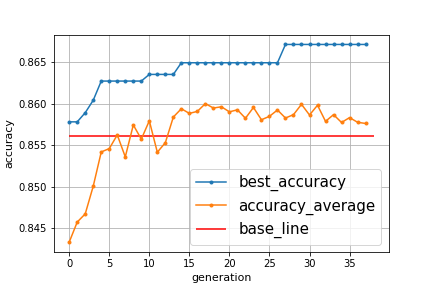
\includegraphics[scale=0.6]{graph1.png}
	\caption{accuracyの推移\label{fig:graph1}}
\end{figure}
最終的な最良値は0.8671となった.
適用確率を追加したとはいえど,1回の学習に使われる枚数自体は4000枚で固定となってしまうので,
前回と大差がないのではないかと考えられる.


\subsection{実験1.2}
実験1.1は前回同様水増ししたものを学習したのに対し,
実験1.2ではgeneratorを用いてミニバッチごとに変換を行った.またこの時元データが2000枚をミニバッチ128枚,31ステップ
で1epochのうち3968枚を学習させる.
\subsubsection{結果}
図\ref{fig:graph2}にaccuracyの最良値及び平均値の推移を示す.
\begin{figure}[hp]
	\centering
	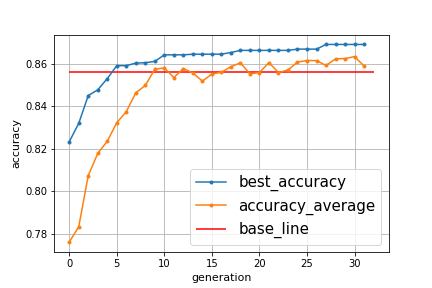
\includegraphics[scale=0.6]{graph2.png}
	\caption{accuracyの推移\label{fig:graph2}}
\end{figure}
最終的な最良値は0.8692となった.実験1.1に比べ改善が見られたかどうかデータの違いが影響したとも考えらえるので
改善したとは言い難い.\\ \\
また,実験時間に関して,1個体の学習時間は実験1.1は90秒,実験1.2は100秒程度であった.またgeneratorを使用しているため,メモリは実験1.2のほうが実験1.1の半分程度に抑えられていた.

\begin{table}[h]
	\centering
	\caption{対照実験\label{tb:taisho}}
	\scalebox{0.9}{
		\begin{tabular}{|c|c|} \hline
			transform&accuracy\\ \hline\hline
			なし(同じ画像二枚ずつ)&0.86043\\ \hline
			shearX&0.8586\\ \hline
			shearY&0.8592\\ \hline
			translateX&0.8628\\ \hline
			translateY&0.8589\\ \hline
			rotate&0.8610\\ \hline
			color&0.8605\\ \hline
			posterize&0.8577\\ \hline
			solarize&0.8313\\ \hline
			constrast&0.8601\\ \hline
			sharpness&0.8606\\ \hline
			brightness&0.8630\\ \hline
			autocontrast&0.8594\\ \hline
			equalize &0.8570\\ \hline
			invert&0.8333\\ \hline
			mirror&0.8624\\ \hline
			flip&0.8366\\ \hline
		\end{tabular}
	}
\end{table}
\section{実験2}
前回のDataAugmentationが有効であるかを示す対照実験として,表\ref{tb:taisho}に各transformに対し変換を行いその結果10回の平均を示す.

だいたいが0.8600前後であり,solarize,invert,flipはあまり良い結果ではないことが分かる.
前回の実験では最良値は0.8676であり,あまり大差がないことが分かる.

\section{今後の課題}
モデルや実験パラメータの改良

\end{document}


